% Author: Izaak Neutelings (June 2017)
% taken from https://tex.stackexchange.com/questions/159445/draw-in-cylindrical-and-spherical-coordinates

\documentclass[border=3pt,tikz]{standalone}
\usepackage{tikz}
\usepackage{tikz-3dplot}
\usepackage{pgfplots}
\tikzset{>=latex} % for LaTeX arrow head
\usetikzlibrary{calc,3d,intersections,positioning,shapes,fillbetween} %,pgfplots.fillbetween

\begin{document}



% 3D
%\tdplotsetmaincoords{-20}{0}
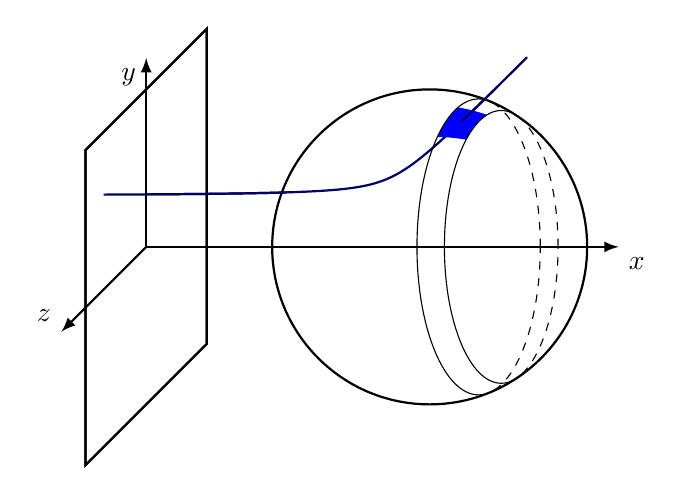
\begin{tikzpicture}
%x={(10mm,0)},y={(0,10mm)},z={(-4mm,-4mm)}
%[scale=1,x={(1,0,0)},y={(0,1,0)},z={(0,0,1)}]
%,x={(10mm,0)},y={(-4mm,-4mm)},z={(0,10mm)}
%,tdplot_main_coords, rotate around x=10

  % variables
  \def\L{6}
  \def\R{2}
  \def\Rz{\R/2.40}
  \def\thetaI{70}
  \def\thetaII{60}
  \def\aI {(\Rz*sin(\thetaI))}  % minor axis
  \def\aII{(\Rz*sin(\thetaII))}
  \def\bI {(\R*sin(\thetaI))}   % major axis
  \def\bII{(\R*sin(\thetaII))}
  \def\dI {sqrt((\bI^2-\aI^2)*(\R^2-\bI^2))/\bI} % ellipse center
  \def\dII{sqrt((\bII^2-\aII^2)*(\R^2-\bII^2))/\bII}
  \def\C{(\L-1.2*\R)} % circle center
  \def\alphaI {atan((\R^2)/(\Rz^2)*cot(\thetaI))}
  \def\alphaII{atan((\R^2)/(\Rz^2)*cot(\thetaII))}
  \def\ellipseI {({\C+\dI},0,0) ellipse ({\aI} and {\bI})}
  \def\ellipseII{({\C+\dII},0,0) ellipse ({\aII} and {\bII})}
  \def\rectangleI {(   0,-\R) rectangle ({\L},{\R})}
  \def\rectangleII{({\C},  0) rectangle ({\L},{\R})}
  
  % trajectory
  \def\tmax{2.2}
  \def\A{0.175*\R}
  \def\B{(0.4*\R)}
  \def\D{sqrt(\A^2+\B^2)}
  \def\N{40} % number of points
  \def\trajectory{
    \draw[thick,black!60!blue,variable=\t,domain=-1.1*\tmax:\tmax,samples=\N,rotate around x=20]
      plot ({-\A/\D*(\A*cosh(\t)+\D) + \B/\D*\B*sinh(\t) + \C},
            { \B/\D*(\A*cosh(\t)+\D) + \A/\D*\B*sinh(\t)});}
  
  
  % axes
  \coordinate (O) at (0,0,0);
  \draw[thick,->] (0,0,0) -- (\L,0,0) node[anchor=north west]{$x$};
  \draw[thick,->] (0,0,0) -- (0,1.2*\R,0) node[anchor=north east]{$y$};
  \draw[thick,->] (0,0,0) -- (0,0,1.4*\R) node[anchor=south east]{$z$};
  \draw[thick] (0,\R,\R) -- (0,\R,-\R) -- (0,-\R,-\R) -- (0,-\R,\R) -- cycle;
  \draw[thick] (0,\R,\R) -- (0,\R,-\R) -- (0,-\R,-\R) -- (0,-\R,\R) -- cycle;
  \trajectory
  
  % sphere (as flat circle)
  %\tdplotdrawarc[thick]{(0,0,{\C})}{\R}{0}{360}{}{}
  \draw[thick]
    ({\C},0,0) circle ({\R});
  %\draw[thick,blue]
  %  ({\C},0,0) ellipse ({\R}  and {\Rz});
  %\draw[thick,blue] ({\C},0,0) ellipse ({\Rz} and {\R} );
  
%  \path[draw,name path=ellipseI]
%    ({\C+\R*cos(\thetaI)},{\R*sin(\thetaI)},0) arc
%    [x radius=\aI,y radius=\bI,start angle={\alphaI},end angle={360-\alphaI}];
%  \path[draw,dashed]
%    ({\C+\R*cos(\thetaI)},{\R*sin(\thetaI)},0) arc
%    [x radius=\aI,y radius=\bI,start angle={\alphaI},end angle={-\alphaI}];
%  \path[draw,name path=ellipseII]
%    ({\C+\R*cos(\thetaII)},{\R*sin(\thetaII)},0) arc
%    [x radius=\aII,y radius=\bII,start angle={\alphaII},end angle={360-\alphaII}];
%  \path[draw,dashed]
%    ({\C+\R*cos(\thetaII)},{\R*sin(\thetaII)},0) arc
%    [x radius=\aII,y radius=\bII,start angle={\alphaII},end angle={-\alphaII}];
  
  % fill area
  \begin{scope}
    \clip \rectangleII; % select first quadrant
    \clip ({\C},0,0) ellipse ({\R} and {0.9*\R});
    \clip[insert path={\rectangleI}]
          ({\C},0,0) ellipse ({\R} and {0.7*\R});
    \clip[insert path={\rectangleI}]
          \ellipseII;
    \fill[blue] \ellipseI;
    %\tikzfillbetween[of=ellipseI and ellipseII] {white!30!blue};
  \end{scope}
  
  % dashed ellipse
  \begin{scope}
    \clip ({\C+\R*cos(\thetaI)},-\R) rectangle ({\L},\R);
    \draw[dashed] \ellipseI;
    \clip ({\C+\R*cos(\thetaII)},-\R) rectangle ({\L},\R);
    \draw[dashed] \ellipseII;
  \end{scope}
  
  % solid ellipse
  \begin{scope}
    \clip ({\C+\R*cos(\thetaII)},-\R) rectangle (0,\R);
    \draw \ellipseII; %[name path global=ellipseI]
    \clip ({\C+\R*cos(\thetaI)},-\R) rectangle (0,\R);
    \draw \ellipseI;  %[name path global=ellipseII]
  \end{scope}
  
  % redraw trajectory
  \begin{scope}
    \clip[insert path={\rectangleI}]
          ({\C},0,0) ellipse ({\R} and {0.81*\R});
    \trajectory
  \end{scope}
  
\end{tikzpicture}





\end{document}